% ============================================================
\chapter{Geodesics and Exponential Map}
\label{ch:geodesics}
% ============================================================

What is the shortest path between two points on a sphere? A great circle, of course. But how does one formulate this question on an arbitrary Riemannian manifold? The answer involves \emph{geodesics}: curves that do not turn, whose covariant acceleration vanishes. On a plane, these are straight lines; on a sphere, great circles; on a surface of revolution, curves computable via the Euler-Lagrange equations of the calculus of variations. The \emph{exponential map}, which sends a tangent vector to the point reached at time 1 along the corresponding geodesic, provides a local coordinate system centred at each point---normal coordinates, where the metric is Euclidean to first order.

\section{The geodesic equation}

\begin{definition}[Geodesic]
Let $(M, g)$ be a Riemannian manifold with Levi-Civita connection $\nabla$.
A smooth curve $\gamma : I \to M$ is a \emph{geodesic} if:
\[
    \nabla_{\dot\gamma}\dot\gamma = 0.
\]
In local coordinates $(x^1, \ldots, x^n)$:
\[
    \ddot\gamma^k(t) + \Gamma^k_{ij}(\gamma(t))\, \dot\gamma^i(t)\, \dot\gamma^j(t) = 0,
    \quad k = 1, \ldots, n.
\]
\end{definition}

\begin{proposition}[Constant speed parametrization]
If $\gamma$ is a geodesic, then $\norm{\dot\gamma(t)}$ is constant. In particular,
geodesics are parametrized proportionally to arc length.
\end{proposition}

\begin{proof}
$\frac{d}{dt}\inner{\dot\gamma}{\dot\gamma} = 2\inner{\nabla_{\dot\gamma}\dot\gamma}{\dot\gamma}
= 0$.
\end{proof}

\begin{theorem}[Local existence and uniqueness]
For every $p \in M$ and $v \in T_pM$, there exists $\varepsilon > 0$ and a unique
geodesic $\gamma_v : (-\varepsilon, \varepsilon) \to M$ with $\gamma_v(0) = p$ and
$\dot\gamma_v(0) = v$.
\end{theorem}

\begin{proof}
The geodesic equation is a second-order ODE system with smooth coefficients.
The Cauchy--Lipschitz theorem guarantees local existence and uniqueness.
\end{proof}

\begin{proposition}[Homogeneity]
For any $\lambda \in \R$ and $v \in T_pM$:
$\gamma_{\lambda v}(t) = \gamma_v(\lambda t)$
wherever both sides are defined.
\end{proposition}

\section{The exponential map}

\begin{definition}[Exponential map]
The \emph{exponential map} at $p \in M$ is:
\[
    \exp_p : \mathcal{D}_p \subset T_pM \to M, \quad v \mapsto \gamma_v(1),
\]
where $\mathcal{D}_p$ is the maximal domain of definition (a star-shaped open set
containing $0$) and $\gamma_v$ is the geodesic with $\gamma_v(0) = p$,
$\dot\gamma_v(0) = v$.
\end{definition}

\begin{proposition}
The map $\exp_p$ is smooth and satisfies:
\begin{enumerate}
    \item $\exp_p(0) = p$.
    \item $(d\exp_p)_0 = \operatorname{Id}_{T_pM}$ (via the canonical identification
          $T_0(T_pM) \cong T_pM$).
    \item $\exp_p(tv) = \gamma_v(t)$ for all $t$ in the domain.
\end{enumerate}
\end{proposition}

\begin{proof}
For (2): $(d\exp_p)_0(v) = \frac{d}{dt}\Big|_{t=0} \exp_p(tv)
= \frac{d}{dt}\Big|_{t=0} \gamma_v(t) = \dot\gamma_v(0) = v$.
\end{proof}

\begin{corollary}
By the inverse function theorem, $\exp_p$ is a diffeomorphism from a neighborhood
of $0$ in $T_pM$ onto a neighborhood of $p$ in $M$.
\end{corollary}

% Exponential map diagram
\begin{center}
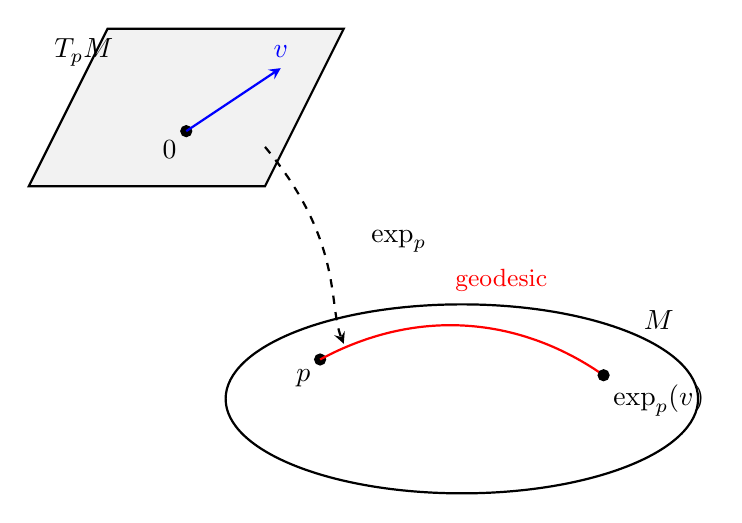
\begin{tikzpicture}[>=stealth, scale=1.0]
  % Tangent plane T_pM (tilted rectangle)
  \fill[gray!10] (-3.5,2.5) -- (-0.5,2.5) -- (0.5,4.5) -- (-2.5,4.5) -- cycle;
  \draw[thick] (-3.5,2.5) -- (-0.5,2.5) -- (0.5,4.5) -- (-2.5,4.5) -- cycle;
  \node at (-2.8,4.2) {$T_pM$};
  % Origin in tangent plane
  \filldraw (-1.5,3.2) circle (2pt) node[below left] {$0$};
  % Vector v in tangent plane
  \draw[->, thick, blue] (-1.5,3.2) -- (-0.3,4.0) node[above] {$v$};
  % Manifold M (ellipse below)
  \draw[thick] (2,-0.2) ellipse (3cm and 1.2cm);
  \node at (4.5,0.8) {$M$};
  % Point p on the manifold
  \filldraw (0.2,0.3) circle (2pt) node[below left] {$p$};
  % Curved geodesic from p to exp_p(v)
  \draw[thick, red] (0.2,0.3) .. controls (1.5,1.0) and (2.8,0.8) .. (3.8,0.1);
  \filldraw (3.8,0.1) circle (2pt) node[below right] {$\exp_p(v)$};
  % Arrow for exp_p
  \draw[->, thick, dashed] (-0.5,3.0) .. controls (0.5,1.8) and (0.3,1.0) .. (0.5,0.5);
  \node at (1.2,1.8) {$\exp_p$};
  % Geodesic label
  \node[red] at (2.5,1.3) {\small geodesic};
\end{tikzpicture}
\end{center}

\section{Normal coordinates}

\begin{definition}[Normal coordinates]
Let $(e_1, \ldots, e_n)$ be an orthonormal basis of $T_pM$. The \emph{normal
coordinates} centered at $p$ are the coordinates $x^i$ defined on a neighborhood
$U$ of $p$ by:
\[
    q = \exp_p(x^1 e_1 + \cdots + x^n e_n).
\]
\end{definition}

\begin{proposition}[Properties of normal coordinates]
In normal coordinates centered at $p$:
\begin{enumerate}
    \item $g_{ij}(p) = \delta_{ij}$.
    \item $\Gamma^k_{ij}(p) = 0$.
    \item $\partial_l g_{ij}(p) = 0$.
    \item Radial geodesics through $p$ are the lines $t \mapsto (tv^1, \ldots, tv^n)$.
    \item The Taylor expansion of the metric is:
          \[
              g_{ij}(x) = \delta_{ij} - \frac{1}{3} R_{ikjl}(p)\, x^k x^l + O(\norm{x}^3).
          \]
\end{enumerate}
\end{proposition}

\begin{proof}
(1) follows from the orthonormal basis choice. (2): radial geodesics satisfy
$\gamma(t) = tv$, so $\ddot\gamma^k = 0$ and the geodesic equation gives
$\Gamma^k_{ij}(p) v^i v^j = 0$ for all $v$, hence $\Gamma^k_{ij}(p) = 0$ by
polarization. (3) follows from (2) and the Christoffel formula.
\end{proof}

\begin{intuition}[title=\textbf{Normal coordinates = linearization of geometry}]
In normal coordinates, the metric is Euclidean to first order: curvature effects
appear only at second order. This is the Riemannian analogue of the fact that
the Earth appears flat locally.
\end{intuition}

\section{The Gauss lemma}

\begin{lemma}[Gauss lemma]
\label{lem:gauss}
Let $p \in M$ and $v \in T_pM$ with $\exp_p(v)$ defined. Then:
\[
    \inner{(d\exp_p)_v(v)}{(d\exp_p)_v(w)} = \inner{v}{w}
\]
for all $w \in T_pM$, identifying $T_v(T_pM) \cong T_pM$.
\end{lemma}

\begin{proof}
Set $q = \exp_p(v)$. The vector $(d\exp_p)_v(v) = \dot\gamma_v(1)$ where
$\gamma_v(t) = \exp_p(tv)$. Consider the variation $F(t,s) = \exp_p(t(v + sw))$.

For fixed $t$, $F(t, \cdot)$ traces radial geodesics. The associated Jacobi
field is $J(t) = \frac{\partial F}{\partial s}\big|_{s=0} = t\, (d\exp_p)_{tv}(w)$.

We compute:
\[
    \frac{d}{dt}\inner{\dot\gamma_v(t)}{J(t)}
    = \inner{\underbrace{\nabla_{\dot\gamma}\dot\gamma}_{=0}}{J}
    + \inner{\dot\gamma}{\frac{DJ}{dt}}.
\]
One shows that $\frac{d}{dt}\inner{\dot\gamma}{J} = \inner{v}{w}$ by noting
$J(0) = 0$ and $\frac{DJ}{dt}(0) = w$. Evaluating at $t = 1$ gives
$\inner{\dot\gamma_v(1)}{J(1)} = \inner{v}{w}$, and since
$J(1) = (d\exp_p)_v(w)$ and $\dot\gamma_v(1) = (d\exp_p)_v(v)$, the result follows.
\end{proof}

\begin{corollary}[Orthogonality of geodesic spheres]
Radial geodesics from $p$ are orthogonal to geodesic spheres
$S(p, r) = \{q : d(p,q) = r\}$ (for $r$ sufficiently small).
\end{corollary}

\section{Minimizing geodesics}

\begin{theorem}[Short geodesics are minimizing]
\label{thm:geod_min}
For every $p \in M$, there exists $\varepsilon > 0$ such that for all
$q \in B(p, \varepsilon)$, there is a unique minimizing geodesic from $p$ to $q$,
and this geodesic is contained in $B(p, \varepsilon)$.
\end{theorem}

\begin{proof}
We use the Gauss lemma and comparison with normal coordinates. Let $\gamma$ be
the radial geodesic from $p$ to $q = \exp_p(v)$ and $\sigma : [0,1] \to M$ any
curve from $p$ to $q$. In normal coordinates, decompose
$\dot\sigma = \dot\sigma^r + \dot\sigma^\perp$ into radial and tangential components
to geodesic spheres. By the Gauss lemma:
\[
    L(\sigma) = \int_0^1 \sqrt{|\dot\sigma^r|^2 + |\dot\sigma^\perp|^2}\, dt
    \geq \int_0^1 |\dot\sigma^r|\, dt \geq |r(1) - r(0)| = \norm{v} = L(\gamma).
\]
\end{proof}

\begin{definition}[Normal neighborhood]
An open set $U \ni p$ is a \emph{normal neighborhood} of $p$ if there is a
star-shaped open set $V \subset T_pM$ containing $0$ such that $\exp_p : V \to U$
is a diffeomorphism and every point of $U$ is joined to $p$ by a unique
minimizing geodesic contained in $U$.
\end{definition}

\section{Injectivity radius}

\begin{definition}[Injectivity radius]
The \emph{injectivity radius} at $p$ is:
\[
    \operatorname{inj}(p) = \sup\{r > 0 : \exp_p|_{B(0,r)} \text{ is a diffeomorphism}\}.
\]
The injectivity radius of $M$ is $\operatorname{inj}(M) = \inf_{p \in M} \operatorname{inj}(p)$.
\end{definition}

\begin{example}[Injectivity radius of $S^n$]
$\operatorname{inj}(S^n) = \pi$: the exponential map ceases to be injective at the
antipodal point.
\end{example}

\begin{example}[Injectivity radius of the flat torus]
For $\mathbb{T}^2 = \R^2/\Z^2$, $\operatorname{inj}(\mathbb{T}^2) = 1/2$.
\end{example}

\begin{example}[Injectivity radius of $\mathbb{H}^n$]
$\operatorname{inj}(\mathbb{H}^n) = +\infty$: the exponential map is a global
diffeomorphism.
\end{example}

\section{Conjugate points and cut locus}

\begin{definition}[Conjugate point]
A point $\gamma(t_0)$ is \emph{conjugate} to $\gamma(0) = p$ along the geodesic
$\gamma$ if $(d\exp_p)_{t_0 \dot\gamma(0)}$ is singular, i.e.\ there exists a
nonzero Jacobi field $J$ along $\gamma$ with $J(0) = J(t_0) = 0$.
\end{definition}

\begin{definition}[Cut point]
The \emph{cut point} of $p$ along $\gamma$ is the first point $\gamma(t_c)$
beyond which $\gamma$ ceases to be minimizing:
\[
    t_c = \sup\{t > 0 : \gamma|_{[0,t]} \text{ is minimizing}\}.
\]
The \emph{cut locus} $\operatorname{Cut}(p)$ is the set of cut points for all
geodesics from $p$.
\end{definition}

\begin{theorem}[Characterization of cut points]
The cut point $\gamma(t_c)$ satisfies one of two conditions:
\begin{enumerate}
    \item $\gamma(t_c)$ is the first conjugate point along $\gamma$.
    \item There exists another minimizing geodesic from $p$ to $\gamma(t_c)$.
\end{enumerate}
\end{theorem}

\begin{example}[Cut locus of $S^n$]
For $p$ the North Pole of $S^n$, $\operatorname{Cut}(p) = \{-p\}$ (the antipodal point).
\end{example}

\section{Geodesics of model spaces}

\begin{example}[Geodesics of $\R^n$]
The geodesics are straight lines: $\gamma(t) = p + tv$.
\end{example}

\begin{example}[Geodesics of $S^n$]
The geodesics are great circles, parametrized by:
$\gamma(t) = \cos(t)\, p + \sin(t)\, v$,
where $p \in S^n$ and $v \in T_pS^n$ with $\norm{v} = 1$.
\end{example}

\begin{example}[Geodesics of $\mathbb{H}^2$ (half-plane)]
The geodesics are:
\begin{itemize}
    \item Vertical half-lines $\{x = x_0, y > 0\}$.
    \item Semicircles centered on the axis $\{y = 0\}$.
\end{itemize}
For a vertical half-line parametrized by $\gamma(t) = (x_0, e^t)$:
$\dot\gamma = (0, e^t)$, $\norm{\dot\gamma}_g = \frac{e^t}{e^t} = 1$, and one
verifies the geodesic equation is satisfied.
\end{example}

\section{Energy functional and first variation}

\begin{definition}[Energy functional]
The \emph{energy} of a curve $\gamma : [a,b] \to M$ is:
\[
    E(\gamma) = \frac{1}{2}\int_a^b \norm{\dot\gamma(t)}^2\, dt.
\]
\end{definition}

\begin{proposition}[Cauchy--Schwarz inequality]
$L(\gamma)^2 \leq 2(b-a)\, E(\gamma)$, with equality if and only if
$\norm{\dot\gamma}$ is constant.
\end{proposition}

\begin{theorem}[First variation formula]
Let $\gamma_s : [a,b] \to M$ be a smooth variation of $\gamma_0 = \gamma$ with
variation field $V = \frac{\partial\gamma_s}{\partial s}\big|_{s=0}$. Then:
\[
    \frac{d}{ds}\bigg|_{s=0} E(\gamma_s) = -\int_a^b \inner{\nabla_{\dot\gamma}\dot\gamma}{V}\, dt
    + \inner{\dot\gamma(b)}{V(b)} - \inner{\dot\gamma(a)}{V(a)}.
\]
\end{theorem}

\begin{corollary}
The critical points of $E$ among curves with fixed endpoints are exactly the
geodesics. Geodesics are thus the \emph{critical curves} of the energy (and length)
functional.
\end{corollary}

\section{Geodesic completeness and Hopf--Rinow}

\begin{definition}
$(M, g)$ is \emph{geodesically complete} if every geodesic can be extended for
all time $t \in \R$.
\end{definition}

We recall that the Hopf--Rinow theorem (Theorem~\ref{thm:hopf_rinow}) establishes
the equivalence between metric completeness and geodesic completeness.

\section{Exercises}

\begin{exercise}
Compute the geodesics of the cylinder $S^1 \times \R$ with the product metric.
Show they are helices (including circles and lines as limiting cases).
\end{exercise}

\begin{exercise}
Show that the geodesics of $\mathbb{H}^2$ in the Poincar\'e disk model are
diameters and circular arcs orthogonal to the boundary $\partial\mathbb{D}$.
\end{exercise}

\begin{exercise}
Let $G = SU(2)$ with a bi-invariant metric. Identify $SU(2) \cong S^3$ and show
that the geodesics are great circles.
\end{exercise}

\begin{exercise}
Compute the injectivity radius of the real projective space $\R P^n$ with the
quotient metric from $S^n$.
\end{exercise}

\begin{exercise}
Show that on a surface of revolution $g = du^2 + f(u)^2 dv^2$, geodesics satisfy
Clairaut's relation: $f^2 \dot v = c$ (constant).
\end{exercise}

\begin{exercise}
Prove the first variation formula for length: if $\gamma$ is arc-length
parametrized:
\[
    \frac{d}{ds}\bigg|_{s=0} L(\gamma_s)
    = -\int_a^b \inner{\nabla_{\dot\gamma}\dot\gamma}{V}\, dt
    + \inner{\dot\gamma}{V}\Big|_a^b.
\]
\end{exercise}
